\xchapter{Metodologia}
{Este capítulo ... }
\label{metodologia}


% IDEIA!
% levantar ano de publicação do artigo para cada software e
% calcular por quanto tempo cada software está disponível,
% com isso verificar se há um padrão, ou seja, se publicações
% mais antigas possuem softwares não-disponíveis, obsoletos,
% etc...

O objeto de estudo é o ecossistema de software acadêmico de análise estática,
ou, ferramentas de análise estática desenvolvidas e publicados na literatura
acadêmica.

A ... em três atividades de (1) busca de artigos
(definição das fontes, obtenção dos artigos nas fontes), (2) filtro (definição
de critérios de busca, definição de script de busca) e (3) seleção de artigos
com publicação de softwares.

o conjunto estudado representa um corte transversal nas
publicações de dois eventos tradicionais da engenharia
de software, análise estática, uma área com um bom histórico

engenharia de software é talvez a área com maior aptidão
para criar softwares, a área de análise estática tem um
histórico maduro, compiladores e afins tem sido foco da
academia desde os princípios dos tempos

o período analisado foi o maior possível, na primeira etapa
de seleção de softwares acadêmicos, o limite foi o número de
edições das conferências selecionadas, optamos por selecionar
conferências ao invés de buscar strings em bibliotecas digitais
por saber a princípio com conhecimento de causa que algumas
conferências tem um alto potencial de encontrar ferramentas

SCAM E ASE, SBES ficou fora :'(

manualmente obtivemos os todos os papers publicados em cada edição
de ambas as conferências

A primeira atividade define as fontes de entrada,
estas fontes são conferências que abordam o tema de interesse do estudo, e
que apresentam um grande potencial de encontrar softwares do domínio de
aplicação desejado, neste estudo o interesse está em softwares de análise
estática de código fonte, portanto as conferências selecionadas serão
aquelas com potencial de se encontrar softwares deste domínio de aplicação.
Esta primeira atividade deve incluir o maior número possível de ediçoes de
cada conferência, para cada edição é copiado localmente todos os artigos em
formato PDF, eles serão utilizados como entrada na atividade 2.

O primeiro passo foi encontrar um conjunto de software acadêmico publicados em
conferências de engenharia de software, duas conferencias foram selecionadas,
SCAM - {\it Source Code Analysis and Manipulation Working
Conference}\footnote{\url{http://www.ieee-scam.org}} e a conferência ASE - {\it
Automated Software Engineering}\footnote{\url{http://ase-conferences.org}},
ambas com um largo histórico de publicação sobre análise de programas e
apresentam um alto potencial de encontrar software do domínio de análise
estática.

%Na revisão estruturada selecionamos a conferência 

Esta seleção foi realizada através de um procedimento composto de 3 (?)
atividades para seleção e coleta de informações sobre software acadêmico de
análise estática. Avaliamos o histórico de publicações de 25 anos da
conferência ASE e 15 anos da conferência SCAM.

\begin{figure}[h]
  \center
  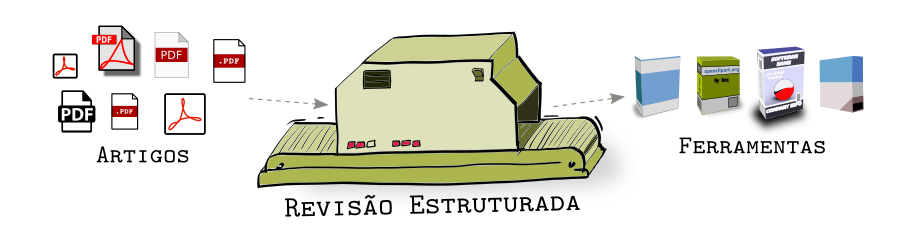
\includegraphics[scale=0.21]{imagens/revisao-estruturada.png}
  \caption{Atividades da revisão estruturada}
  \label{figura-revisao-estruturada}
\end{figure}

As 3 atividades da revisão estruturada, representadas na Figura
\ref{figura-revisao-estruturada}, apresentam como resultado final um conjunto
de softwares com as seguintes informações:

\begin{itemize}
  \item Nome e descrição do software acadêmico.
  \item Título do artigo onde o software é citado como contribuição, seja principal ou secundária.
  \item Nome e ano da conferência onde o artigo foi publicado.
  \item Endereço onde o software pode ser obtido, páginas web ou repositórios de código fonte.
\end{itemize}

Cada atividade da revisão gera como saída um conjunto de artigos, este conjunto
é reduzido a cada atividade, a última delas gera também um conjunto de
softwares acadêmicos com algumas de suas informações.

A primeira atividade -- (1) Busca -- passa por todas as ediçoes das
conferências até o ano de 2015, incluindo as publicações de 2015.  Exploramos o
histórico de 24 anos de publicação dessas conferências.

As informações coletadas sobre cada software inclui nome, descrição e o
endereço onde obter uma cópia, normalmente página web ou repositório de código
fonte, esses endereços foram verificados para confirmar se os softwares estão,
de fato, disponíveis, parte dos dados coletados coincidem com o trabalho
recente, publicado após o início deste estudo, \cite{howison2016software}, o
autor sugere um esquema de codificação para menções a software:


\begin{minipage}[t]{0.3\textwidth}
bla
\end{minipage}

\begin{table}[h]
\caption{Coding scheme for mentions of software \cite{howison2016software}}
\centering
\begin{tabular}{ l p{8cm} }
  \hline
  Código                   & Definição \\
  \hline
  Nome do software         & O nome do projeto de software \\
  URL                      & Endereço web do software ou projeto \\
  Número de versão         & Um número de versão (ou tag no código fonte) identificando uma versão específica do software \\
  Data                     & Uma data usada para indicar uma versão do software (não é a data do artigo ou referência) \\
  Detalhes de configuração & Qualquer menção a configuração do software \\
  Software utilizado       & Para menções ao software que foi utilizado na pesquisa \\
  Software não utilizado   & Para menções ao software que os autores não \\
                           & utilizaram (ex, discute-se porque não utilizou \\
                           & um determinado software, ou o método implementado pelo software) \\
  Criador                  & Menção ao criador do software (pode ser aplicado no texto ou nas referências) \\
  \hline
\end{tabular}
\label{coding-scheme-mentions}
\end{table}


Diferentemente do autor do esquema na tabela \ref{coding-scheme-mantions} nós
estamos lidando apenas com software publicado junto ao paper selecionado, ou seja,
selecionamos artigos publicando software como contribuição da pesquisa, sem distinguir
entre cintribuição principal do estudo ou secundária.

Desta forma coletamos apenas Nome e URL, o campo Criador será os mesmos
criadores do artigo onde o software foi publicado. Os demais campos não foram coletados uma
vez que não estamos capturando publicações que apenas utilizaram software acadêmico, mas
sim aquelas que tenham criado, ou ao menos contribuido, mas que descrevem
no texto que o software ou ferramenta é uma contribuição.

A segunda atividade -- (2) Filtro -- reduz o número total de artigos de forma
automática a partir da seguinte {\it string} de busca.  A segunda atividade
realizada em cima de todo o conjunto de artigos selecionados na etapa anterior
é uma busca pelos seguintes termos em todo o conteúdo dos artigos:

\begin{verbatim}
  "tool" OU "framework"; E
  "download" OU "available"; E
  "http" OU "ftp"; E
  "static analysis" OU "parser".
\end{verbatim}

Esses termos devem ser pensados em relaçao ao domínio de aplicação
desejado, devem ser abrangentes a fim de evitar falsos negativos, ou seja,
evitar que o filtro deixe de fora artigos que publiquem software de análise
estática, mesmo que isto resulte em falsos positivos, a atividade seguinte
identificará esses falsos negativos deixando-os fora do resultado final.

Esses termos devem encontrar artigos com publicação de softwares
científicos do domínio de análise estática de código fonte com
disponibilidade para {\it download}, seja binário ou código fonte, será
aplicado automaticamente com auxílio de um script desenvolvido durante este
trabalho de pesquisa, detalhes deste script, outros artefatos produzidos
durante esta pesquisa, e onde obtê-los pode ser encontrado no Apêndice
\ref{reproducibilidade-do-estudo}.

A terceira e última atividade identifica se cada
artigo resulta, de fato, em publicação de software acadêmico de análise
estática. Esta seleção é feita a partir de uma leitura superficial do
artigo em busca de indícios de que o artigo publica de fato algum software.

Essa leitura inclui título, introdução, resultados e conclusões, o objetivo
é identificar se o artigo publica software acadêmico e indica onde obter
uma cópia do software. Quando esta leitura inicial não é o suficiente para
identificar se há publicação de software, outras seções são lidas, alguns
artigos descrevem a implementação do software em seções específicas, outros
indicam detalhes do software ao longo do texto, é comum o uso de
notas de rodapé para indicar onde o software está disponível. Software
acadêmico que seja mais abrangente do que apenas análise estática de
código fonte mas que contenham esta função em seu conjunto também são
selecionados.

A seleção de softwares acadêmicos foi realizada através de um procedimento
inspirado na revisão e no mapeamento sistemático de literatura, chamado de
revisão estruturada, composto de atividades para seleção e coleta de
informações sobre softwares acadêmicos de análise estática, essa revisão
avaliou o histórico de publicações de 25 anos da conferência ASE e 15 anos da
conferência SCAM.

As informações coletadas sobre cada software inclui nome, descrição e o
endereço onde obter uma cópia, normalmente página web ou repositório de código
fonte, esses endereços foram verificados para confirmar se os softwares estão,
de fato, disponíveis.

Em \cite{howison2016software} também coletamos informações similares ao esquema
proposto para coletar características do próprio software (Tabela
\ref{codes-for-functions}):

\begin{table}[h]
\caption{Codes for functions \cite{howison2016software}}
\centering
\begin{tabular}{ l p{8cm} }
  \hline
  Código                          & Explicação \\
  \hline
  Identificável                   & Podemos identificar qual software foi mencionado (ex, Existe um nome, ... "um programa que nós escrevemos?" Podemos encontrar referencias para o software, mesmo que o software não seja encontrado?) \\
  Encontrável                     & Dado uma peça de software identificável, podemos encontrar uma fonte online que detalha o software (não necessariamente o próprio software, mas alguma presença oficial) (ex, a página do projeto ou manual online)? \\
  Versão encontrável              & Podemos encontrar uma versão específica listada no artigo, se sim, qual? \\
  Acesso                          & Podemos acessar o software agora? Pode receber os seguintes valores: Sem Acesso, Acesso Pago, Acesso Gratuito \\
  Código disponível               & É possível acessar o código fonte de alguma forma? \\
  Permissão para modificar        & Os criadores dão permissão para modificar o programa (se não menciona modificação, assume não)?; se permissão apenas por contato, também não \\
  Corresponde à citação preferida & Se a página do projeto lista uma maneira preferida de citação ao software, se sim, a menção encontrada no artigo casa com essa preferência? \\
  \hline
\end{tabular}
\label{codes-for-functions}
\end{table}

apesar de ter coletado não coletamos apenas citações formais, qualquer citação,
sem distinção, desde que deixe aparente que o artigo utiliza o software a citação
é coletada e o paper marcado como um do conjunto de citações daquele software

usei a tabela TABLE 5 do trabalho de howison2016software na revisao estruturada
na fase de coleta (adaptar depois), mas n preciso usar o campo Identifiable, pois
a revisao estruturada só retorna softwares assim, mas na sequencia eu uso os
mesmo dados, com nomes diferente, basta eu adaptar meu texto e dados para casar,
Findable, Access, Source available, Permission to modify, Matches preferred citation eu
não coletei, mas n sei se é interessante pro meu caso, talvez sim, ou não...

características da menção aos softwares

com base numa adaptação de \cite{howison2016software} identificamos as caracteristicas
da tabela abaixo em cada menção encontrara nas menções

* nome do software, toda citação tem nome pois foi através do nome que buscamos as citações
* tipo e peso da citação (peso em ordem crescente)
cita
  - apenas cita o software ou é o mesmo artigo selecionado na revisão estruturada
  - ou é um artigo com "mesmo" conteúdo publicado na "mesma" época \^
  - descreve o software
  - cita numa tabela com outros, classifica
  - cita como exemplo
  - cita trabalho relacionado
  - cita em trabalhos futuros
avalia ou usa
  - avalia ou caracteriza o software
  - usa para coleta ou análise de dados
  - usa como objeto de estudo
  - usa o software como parte de uma solução, implementação, etc
  - cria um software derivado mas não disponibiliza as contribuições
contribui
  - contribuição pequena ou moderada
  - extende o software
  - integra o software a outros sistemas, formatos de entrada/saída, APIs, etc
    (seja implementando suporte no software ou do outro lado)
  - refatora parte do software
  - implementa parte do software em outro projeto e compara resultados
cria ou CONTRIBUI
  - contribuição inicial criando o projeto
  - faz uma grande contribuição
  - refatora todo o software
  - abre o código

Os softwares disponíveis foram avaliados em relação à disponibilidade de código
fonte e à licença utilizada, essas informações, e as demais coletadas até aqui,
foram distribuídas cronologicamente, e interpretadas numa perspectiva histórica
sobre a sustentabilidade técnica dos softwares acadêmicos de análise estática.

Os softwares disponíveis foram avaliados em relação à disponibilidade de código
fonte e à licença utilizada, essas informações, e as demais coletadas até aqui,
foram distribuídas cronologicamente, e interpretadas numa perspectiva histórica
sobre a sustentabilidade técnica dos softwares acadêmicos de análise estática.


%%%%%%%%%%


No segundo estudo, os softwares com código fonte disponível foram avaliados em
relação a sua manutenabilidade através da métrica de complexidade estrutural. A
coleta dessa métrica para cada software foi realizada pelo Analizo, uma suíte
de ferramentas para análise de código fonte, e está sendo considerado como um
indicador de manutenabilidade.


um conjunto total de  XXX artigos, tabela e figura com a distribuicao
dos artigos

obtivemos o arquivo pdf de cada paper

nosso conjunto de seleção incluindo todas publicações de conferência
nos permite ter uma visão do histórico de publicações de softwares
acadêmicos nestes eventos

(seleção estruturada gera lista de softwares academicos de origem cientifica de analise estatica)

secao: identificando menção aos softwares acadêmicos selecionados


4º Princípio, Persistencia

Os identificadores únicos e metadados descrevendo o software e sua disposição
devem persistir - mesmo além do tempo do software que descrevem.

Acesso ao software

5º Princípio da citação à softwares, Acessibilidade:

``citações aos softwares devem permitir e facilitar acesso ao software,
metadados, documentação, dados e outros materiais necessários tanto
para humanos quanto para máquinas se informar do referido software''

Não significa que o software deva estar disponível gratuitamente, mas que
os metadados devem prover informação suficiente para que o software seja
acessado. Se o software é livre, os metadados devem prover um identificador
que pode ser resolvido para uma URL apontando para a versão específica
do software sendo citado.

Pra softwares comerciais, os metadados devem ainda prover informações sobre
como acessa o software, mas pode ser um número de telefone da empresa que
vende o software ou o link para um site que venda o software

\cite{smith2016software}

5. Accessibility: Software citations should facilitate access to the software itself and to its


o próximo passo coletamos os nomes dos autores de cada artigo que faz menção
aos softwares em nosso conjunto, os nomes dos autores foram normalizados,
e para cada artigo citando um software extraimos e identificamos o nível
de ineditismo daqueles pesquisadores com aquele software, os valores
são os seguites:

escala de peso da autoria:
==========================

são os primeiros autores a publicar sobre o software
  authorship\_weight=0
todos os autores já publicaram sobre o software em anos anteriores
  authorship\_weight=0.1
uma parte dos autores já publicou sobre o software em anos anteriores
  authorship\_weight=0.25
nenhum dos autores jamais publicou sobre o software
  authorship\_weight=0.5



análise estática


====



aartigo propoe uma categoria de tipos de citacao a softwares,
coincide com o que eu coletei, posso usar algumas dimensoes
\cite{smith2016software}

cada citação pontua no máximo 1 ponto para o peso final do paper ao quanto
contribui para a sustentabilidade técnica do software, esta pontuação será
calculada com base nos pesos (em porcentagem) 'contribution\_weight' e
'authorship\_weight', este último valor é aplicado à contribution weight,
ou seja contribution\_weight é acrescido a partir do valor de authorship\_weight.
o valor final se ultrapassar 1 será cortado no limite 1 (máximo), a ideia não é muito
os números, não queremos saber se são numeros altos, queremos constancia, queremos
medir se existe um nível de contribuição mínimo aos softwares, isto está
sendo proposto como algo que mantém o software vivo e útil para a comunidade
acadêmmica. (por hora o valor mínimo "ideal" por ano é "0.5", ou seja, um
valor bem modesto, este valor indica que houve ao menos uma contribuição
ao software, ou que teve citações suficientes equivalente a uma contribuição,
o software ao ser muito citado ganha mais visibilidade, impacta na possibilidade
de maior adoção e maior contribuição por terceiros.

outro fator de peso para definir o valor final do peso é se houve lençamentos
de novas versões do software naquele ano, se houve ao menos 1 versão lançada,
isso leva o final\_weight para o valor máximo 1.0 (que representa 100\%)

* revisão estruturada
   paper{step} = 'structured-review';
* citações ao software
   citations{key}{step} = 'review-citations';

escala de peso da contribuição:
===============================

cita
  contribution\_weight=0.1
avalia ou usa
  contribution\_weight=0.25
contribui
  contribution\_weight=0.5
cria ou CONTRIBUI
  contribution\_weight=1

contribuições sem peso:
=======================

o software mudou de nome, qual o nome antigo, qual o novo nome
um novo software foi criado a partir daqui, qual o nome do novo
um novo software foi criado com base neste

  weightless\_contributions={},

%####

%#### artigos nao encontrados para download:
%
%  url = {http://doi.acm.org/10.1145/3090064.3090070},
%
%#### para instalar a versão correda do analizo:
%
%apt-get install doxyparse=1.8.11 analizo=1.19.1


%
% Metodologia
%
%No segundo estudo, os softwares com código fonte disponível foram avaliados em
%relação a sua manutenabilidade através da métrica de complexidade estrutural. A
%coleta dessa métrica para cada software foi realizada pelo Analizo, uma suíte
%de ferramentas para análise de código fonte, e está sendo considerado como um
%indicador de manutenabilidade.
%
%Um conjunto de softwares de análise estática da indústria foi incluído nesta
%etapa, todos os dados coletados para os softwares acadêmicos foram também
%coletados para este novo conjunto. Esses softwares foram então caracterizados em
%relação à frequencia de lançamentos, linguagem de programação e o tipo de
%entrada suportado.
%
%Todas estas características foram comparadas entre sí, por exemplo, softwares
%com maior frequencia de lançamentos, escritos na mesma linguagem de
%programação, apresentam maior complexidade estrutural? Eles são da academia ou
%da indústria? Softwares da indústria apresentam melhor manutenabilidade do que
%os softwares acadêmicos?
%
%Essas perguntas serão respondidas através de uma análise exploratória dos
%dados, essa análise apresenta também uma perspectiva evolutiva de alguns
%softwares, aqueles com maior frequencia de lançamentos foram selecionados para
%esta avaliação.
%
%(continua...)

%como essas taxas mudam ao longo do tempo.
%
%Dessa forma, definimos como objetivo geral deste trabalho medir a qualidade
%(técnica e não-técnica) dos softwares acadêmicos de origem científica da
%engenharia de software e explorar como essas taxas mudam ao longo do tempo.
%
%Questão de pesquisa:
%
%* Como ocorre o co-desenvolvimento dos softwares
%* Como acontece colaboração na construção dos softwares
%* Como os softwares contribuem para a construcao de conhecimento novo em novas pesquisas derivadas
%
% * mais da metade desenvolvem seus próprios softwares
% * falta de visibilidade gera questionamentos sobre qualidade
% * falta de treinamento leva a produzir softwares sem qualidade
% * produtividade científica requer capacidade de replicação
% * capacidade de replicação depende de qualidade

\subsection{Software acadêmico de análise estática}

Os softwares avaliados neste estudo serão do domínio de aplicação de análise de
código-fonte, ...
